%===============================================
%
% Friggeri-CV-Modified  
% Version 1.1 (11/04/2015)
%
% This work is based on a LaTex template that was originally created by % Adrien Friggeri and that has later been modified by LaTeXTemplates.
%
% Copyright (C) 2015 Jean-Sébastien Gosselin
% https://github.com/jnsebgosselin/Curriculum-Vitae
%
% Copyright (C) 2014 LaTeX Templates
% http://www.LaTeXTemplates.com
%
% Copyright (C) 2012 Adrien Friggeri (adrien@friggeri.net) 
% https://github.com/afriggeri/CV
%
% This work is free software: you can redistribute it and/or modify it under the terms of the CC BY-NC-SA 3.0 License as published by the Creative Commons nonprofit organization.
%
% This work is distributed in the hope that it will be useful, but WITHOUT ANY WARRANTY; without even the implied warranty of MERCHANTABILITY or FITNESS FOR A PARTICULAR PURPOSE. See the CC BY-NC-SA 3.0 License for more details at http://creativecommons.org/licenses/by-nc-sa/3.0/.
%
% Important notes:
% This template needs to be compiled with XeLaTeX and the bibliography, if used, needs to be compiled with biber rather than bibtex.
%
%===============================================

\documentclass[print]{friggos-cv} % Add 'print' as an option into the square bracket to remove colors from this template for printing

\usepackage{afterpage} % to change the geometry of pages
\usepackage{array}     % To add extra row height to tabular
\usepackage{graphicx}  % to include images
\usepackage{enumitem}  % control left margin of itemize environment

%---- Add Page Number at the bottom right of the page ----

\usepackage{fancyhdr}
% Turn on the style
\pagestyle{fancy}
% Clear the header, footer, and rules
\fancyhf{}
\renewcommand{\headrulewidth}{0pt}
% Set the right side of the footer to be the page number
\fancyfoot[R]{page \thepage}
% Offset the footer to take into account the aside environment width
\fancyfootoffset[RO]{5.25cm}

\begin{document}

\header{John}{Doe}{junior business analyst} % Your name and current job title/field

%-----------------------------------------------
%	SIDEBAR SECTION (first page)
%-----------------------------------------------

\begin{aside} % In the aside environment, each new line forces a line break
	\section{contact}%
	    \vspace{5pt}
		\home\space 2020 des Sapins, \#123
		\hspace{0.43cm}City, State, Country
		\hspace{0.43cm}G3C 4T3\vspace{5pt}
		\phoneb \space (123) 456 7890
		\href{}{\mail\space john@doe.com}
		\vspace{10pt}%
	\section{about}%
		\vspace{5pt}
		age
		nationality
		 marital status, nbr. of kids%
		\vspace{5pt}
		\href{}{\globe\hspace{0.1cm} http://www.johndoe.ca}
		\href{}{\linkedin\hspace{0.1cm} LinkedIn: johndoe}
		\href{}{\facebook\hspace{0.1cm} Facebook: johndoe}
		\href{}{\github\hspace{0.1cm} GitHub: johndoe}
		\vspace{10pt}%
	\section{langues}%
		\vspace{5pt}
		First Language (native)
		Second Language (current)
		\vspace{10pt}%
	\section{professional interests}%
		\vspace{10pt}
		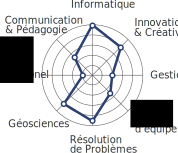
\includegraphics[width=4.5cm]{prof_interests_graph}
		\vspace{5pt}%
	\section{programmation}%
		\vspace{-5pt}
		{%
		\setlength{\extrarowheight}{2pt}%
		\begin{tabular}{@{}m{2cm}m{2.5cm}@{}}
			Python 2.7 & \hfill \skillScale{4}
			Matlab     & \hfill \skillScale{3}
			LabView    & \hfill \skillScale{2}
			\LaTeX     & \hfill \skillScale{3}
			HTML       & \hfill \skillScale{1}
			Fortran 95 & \hfill \skillScale{1} 
		\end{tabular}%
		}
\end{aside}
%{\color{red} $\varheartsuit$}

%-----------------------------------------------
%	SUMMARY SECTION
%-----------------------------------------------

\section{summary}
%
\normalfont{Lorem ipsum dolor sit amet, consectetur adipiscing elit, sed do eiusmod tempor incididunt ut labore et dolore magna aliqua. Ut enim ad minim veniam, quis nostrud exercitation ullamco laboris nisi ut aliquip ex ea commodo consequat.}

%-----------------------------------------------
%	EDUCATION SECTION
%-----------------------------------------------

\section{education}

\begin{entrylist}
%------------------------------------------------
\entryMod
{2010--Prés.}
{PhD {\normalfont Program of Study}}
{Institution Name}
{Research project - field of study}
{Lorem ipsum dolor sit amet, consectetur adipiscing elit, sed do eiusmod tempor incididunt ut labore et dolore magna aliqua. Ut enim ad minim veniam, quis nostrud exercitation ullamco laboris nisi ut aliquip ex ea commodo consequat.}
%------------------------------------------------
\entryMod
{2007--2009}
{MScA {\normalfont Program of Study}}
{Institution Name}
{Research project - field of study}
{Lorem ipsum dolor sit amet, consectetur adipiscing elit, sed do eiusmod tempor incididunt ut labore et dolore magna aliqua. Ut enim ad minim veniam, quis nostrud exercitation ullamco laboris nisi ut aliquip ex ea commodo consequat.}
%------------------------------------------------
\entryMod
{2002--2006}
{Bing {\normalfont Program of Study}}
{Institution Name}
{Final project study - field of study}
{Lorem ipsum dolor sit amet, consectetur adipiscing elit, sed do eiusmod tempor incididunt.}
%------------------------------------------------
\entryAlt
{2000--2002}
{DEC {\normalfont Program of Study}}
{Institution Name}
%------------------------------------------------
\end{entrylist}


%-----------------------------------------------
%	WORK EXPERIENCE SECTION
%-----------------------------------------------

\section{experience}

%------------------------------------------------
\begin{entrylist}
  \entryBul
    {2010--Prés.}
    {Employer Name}
    {city, province, country}
    {position occupied - field of study}
    {
     \begin{itemize}[leftmargin=*]
       \setlength\itemsep{0pt}
       \item Lorem ipsum dolor sit amet, consectetur adipiscing elit, sed do eiusmod tempor incididunt.                     
       \item Lorem ipsum dolor sit amet, consectetur adipiscing elit:
         \begin{itemize}[leftmargin=0.5cm]
           \item Lorem ipsum dolor sit amet, consectetur adipiscing elit.
           \item Lorem ipsum dolor sit amet, consectetur adipiscing elit.
         \end{itemize}
       \item Lorem ipsum dolor sit amet, consectetur adipiscing elit, sed do eiusmod tempor incididunt.
       \item Lorem ipsum dolor sit amet, consectetur adipiscing elit, sed do eiusmod tempor.
       \item Lorem ipsum dolor sit amet, consectetur adipiscing elit, sed do eiusmod tempor incididunt ut labore et dolore magna aliqua.
     \end{itemize}
     }
\end{entrylist}
%------------------------------------------------
\begin{entrylist}
  \entryBul
    {05-09 2005}
    {Employer Name}
    {city, province, country}
    {position occupied - field of study}
    {
     \begin{itemize}[leftmargin=*]
       \setlength\itemsep{0pt}
       \item Lorem ipsum dolor sit amet, consectetur adipiscing elit, sed do eiusmod tempor incididunt.
       \item Lorem ipsum dolor sit amet, consectetur adipiscing elit, sed do eiusmod tempor incididunt ut labore et dolore magna aliqua.
     \end{itemize}
     }
\end{entrylist}
%------------------------------------------------
\begin{entrylist}
  \entryBul
    {09-12 2004}
    {Employer Name}
    {city, province, country}
    {position occupied - field of study}
    {
     \begin{itemize}[leftmargin=*]
       \setlength\itemsep{0pt}
       \item Lorem ipsum dolor sit amet, consectetur adipiscing elit.
       \item Lorem ipsum dolor sit amet, consectetur adipiscing elit, sed do eiusmod tempor incididunt.
     \end{itemize}
     }
\end{entrylist}

%-----------------------------------------------
%	CERTIFICATION SECTION
%-----------------------------------------------
\newpage
\section{certifications}
  \begin{entrylist}
    \entryFULL
      {2014--Prés.}
      {Certification Authority}
      {}
      {Certification Name - Licence xxxxxx}
      {}
%------------------------------------------------
    \entryFULL
      {2003--Prés.}
      {Certification Authority}
      {}
      {Certification Name - Licence xxxxxx}
      {}
\end{entrylist}

%-----------------------------------------------
%	COMMUNICATION SKILLS SECTION
%-----------------------------------------------

%\newgeometry{left=1.5cm,top=2cm,right=1.5cm,bottom=2cm,nohead,nofoot}

\section{notable communication}
\textbf{\large written}\vspace{10pt}\\
\begin{entrylist}
%------------------------------------------------
\entry
{in prep.}
{Lorem ipsum dolor sit amet, consectetur adipiscing elit, sed do eiusmod tempor incididunt.}
{}
{author name, author name, author name et author name\\\emph{Journal Title and Info}}
%------------------------------------------------
\entry
{AOÛ 2010}
{Lorem ipsum dolor sit amet, consectetur adipiscing elit, sed do eiusmod tempor incididunt.}
{}
{author name, author name, author name et author name\\\emph{Journal Title and Info}}
%------------------------------------------------
\end{entrylist}
\textbf{\large oral and posters}\vspace{10pt}\\
\begin{entrylist}
%------------------------------------------------
\entry
{MAI 2015}
{Lorem ipsum dolor sit amet, consectetur adipiscing elit, sed do eiusmod tempor incididunt.}
{}
{author name, author name, author name et author name\\\emph{Presentation Type (Language), Conference Title, Location, City}}
%------------------------------------------------
\entry
{MAI 2014}
{Lorem ipsum dolor sit amet, consectetur adipiscing elit, sed do eiusmod tempor incididunt.}
{}
{author name, author name, author name et author name\\\emph{Presentation Type (Language), Conference Title, Location, City}}
%------------------------------------------------
\end{entrylist}

%-----------------------------------------------
%%	SIDEBAR SECTION (Second Page)
%-----------------------------------------------

\begin{aside2}
    \section{softwares}
	    \parbox[t]{4.5cm}{{\footnotesize\emph{Interest and ability to learn new software high}}}
	    \vspace{10pt}%
	    {\addfontfeature{Color=lightgray}Office}%
	    \vspace{-8pt}
	    \begin{tabular}{@{}m{2.4cm}m{2.1cm}@{}}
	        LibreOffice & \hfill \skillScale{4}
	        MS Office   & \hfill \skillScale{3}
	        Zotero      & \hfill \skillScale{4}
	        Thunderbird & \hfill \skillScale{4}
	    \end{tabular}    
	    \vspace{-6pt}%
	    {\addfontfeature{Color=lightgray}Graphic Design}%
	    \vspace{-6pt}
	    \begin{tabular}{@{}m{2.4cm}m{2.1cm}@{}}
	        Inkscape & \hfill \skillScale{3}
	        GIMP     & \hfill \skillScale{2}
	        MS Visio & \hfill \skillScale{3}
	        Scribus  & \hfill \skillScale{2}
	    \end{tabular}
	    \vspace{-6pt}%
	    {\addfontfeature{Color=lightgray}Operating Systems}%
	    \vspace{-6pt}
	    \begin{tabular}{@{}m{2.4cm}m{2.1cm}@{}}
	        Linux   & \hfill \skillScale{4}
	        Windows & \hfill \skillScale{3}
	    \end{tabular}    
	    \vspace{-6pt}%
	    {\addfontfeature{Color=lightgray}Specialized Software}%
	    \vspace{-6pt}
	    \begin{tabular}{@{}m{2.4cm}m{2.1cm}@{}}
	        ArcGIS & \hfill \skillScale{2}
	        \footnotesize{Visual MODFLOW} & \hfill \skillScale{1}
	        Tecplot & \hfill \skillScale{1}        
	    \end{tabular}        
        \vspace{-5pt}%
    \section{personal interests}%
        \vspace{10pt}
        Music, reading,
        Open Source Softwares,
        New Technologies,
        Badminton et Bicycle
\end{aside2}


\end{document}
